\documentclass[a4paper]{article}

\usepackage[latin1]{inputenc} 
\usepackage{graphicx}
\usepackage{natbib}
\usepackage{amsmath}
\usepackage{subcaption}

\usepackage{listings}
\usepackage{color}

% \usepackage{draftwatermark}
%\usepackage{fullpage}

% \SetWatermarkText{
\includegraphics{sw_logo.png}}
\newcommand{\bm}[1]{\mbox{\boldmath{$#1$}}}

\definecolor{codegreen}{rgb}{0,0.6,0}
\definecolor{codegray}{rgb}{0.5,0.5,0.5}
\definecolor{codepurple}{rgb}{0.58,0,0.82}
\definecolor{backcolour}{rgb}{0.95,0.95,0.92}

\lstdefinestyle{mystyle}{
    backgroundcolor=\color{backcolour},   
    commentstyle=\color{codegreen},
    keywordstyle=\color{magenta},
    numberstyle=\tiny\color{codegray}, 
    stringstyle=\color{codepurple},
    basicstyle=\footnotesize,
    breakatwhitespace=false,         
    breaklines=true,                 
    captionpos=b,                    
    keepspaces=true,                 
    numbers=left,                    
    numbersep=5pt,                  
    showspaces=false,                
    showstringspaces=false,
    showtabs=false,                  
    tabsize=2
}
 
\lstset{style=mystyle}




\begin{document}

\begin{center}
%
\includegraphics[width=0.2\textwidth]{sw_logo} \\
\vspace{0.5 cm}
\huge{\textbf{PlantBox: RootSystem Tutorial}} \\
\vspace{0.5 cm}
\normalsize
Daniel Leitner @ SimWerk \\
www.simwerk.at 
\end{center}

\vspace{0.5 cm}

\noindent 
The following tutorial offers scripts to outline the usage of the CPlantBox Python binding named \emph{plantbox} for many different applications. CPlantBox was developed from CRootBox and is largely backward compatible by having the same underlying rootsystem model. For further documentation please refer to the Doxygen class documentation of the CPlantBox code.


\vspace{0.5 cm}

\tableofcontents

\newpage

\section{Basic usage} /label{sec:basic}

\subsection{Installation notes}

After successfully compiling CPlantBox the Python library \emph{plantbox} should be available on the system. 
Additionally, you will need the following Python packages: numpy, scipy, matplotlib, and vtk (e.g. pip3 install numpy). 

The figures of the rootsystem were created using Paraview, and some Paraview Python scripts for convenience.
% TODO

\subsection{Small example}

The first example shows how to use CPlantBox: open a parameter file (L12), do the simulation (L18), 
save the result (L21), and make an interactive plot showing the results (L24). 

\lstinputlisting[language=Python, caption=Example 1a]{../../examples/python/example1a_small.py} 

\noindent 
Lets revise the above code in more detail: 
\begin{itemize}
 \item[2,3] We add the path to py\_plantbox.
 \item[3] Imports the CPlantBox Python library (py\_plantbox) and name it pb.
 \item[4] Imports a auxilliary script for visualization of the rootsystem with vtk
 \item[7] Constructs the root system object.
 \item[12] Opens an .xml containing parameters describing the types of root (RootRandomParameters), 
 and the type of pant (SeedRandomParameters). Alternatively, all parameter can be set or modified directly in Python 
 (see Section \ref{sec:sa}).
 \item[15] Initializes the simulation: Creates the tap root the base roots 
 (i.e. all basal roots, and shoot borne roots that might emerge), creates the tropisms and passes the domain geometry to it, 
 and creates the elongation functions. 
 \item[18] Performs the simulation. The value 30 is the simulation time in days. 
 If no simulation time is passed the simulation time is taken from the .pparam file. 
 Note that simulation results are independent from the time step, i.e. 30 simulate(1) calls should yield the same result 
 as simulate(30). 
 \item[21] Saves the resulting root system geometry in the VTK Polygonal Data format (VTP) as polylines, 
 see Figure \ref{fig:basicA}. 
 \item[24] Create an interactive plot (use mouse to rotate or zoom) using VTK. 
 Per default 'creationTime', 'radius', or 'type' can be viusalized.
 You can save a screenshot as png file by pressing 'g'.
 \end{itemize}
  
\subsection{Growth in a container}

This is an extension of the previous example, where the root system grows in one of two containers 
(a soil core or rectangular rhizotron). Such geometries are important if we want to mimic experimental settings. 
In CPlantBox the domain geometry is represented in a mesh free way using signed distance functions (SDF). 
A SDF returns the distance to the closest boundary, with negative sign if it lies inside of the domain, 
and a positive if the point is outside.

\lstinputlisting[language=Python, caption=Example 1b]{../../examples/python/example1b_container.py}

The geometry is first created by constructing some specialization of the class SignedDistanceFunction, 
and is passed to the root system by the method setGeometry: 
\begin{itemize}
 \item[17] Construct a soil core. 
 \item[20] Construct a rhizotron.
 \item[23] Pick one of the two geometries. Note that it is important to call setGeometry before initialize.
 \item[35] Its possible to save the geometry as Paraview Python script for visualization (and debugging) in Paraview, 
 see Figure \ref{fig:basicB}. Run this script in Paraview by Tools$\rightarrow$Python Shell, Run Script.
\item[35] The geometric boundaries can currently not be visualized in the interactive rendering 
This could be achieved in VTK by creating an iso-surface of the implicit geometry given by the SDF.
\end{itemize}

\begin{figure}
\begin{subfigure}[c]{0.5\textwidth}
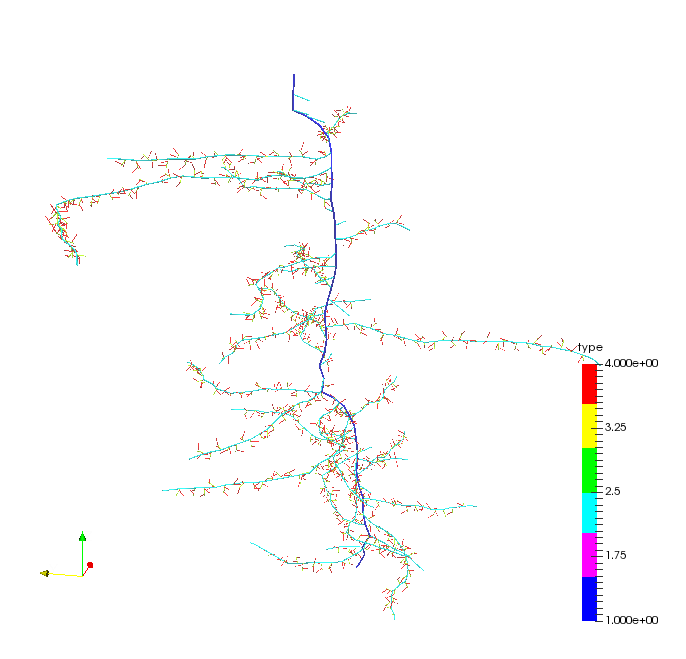
\includegraphics[width=0.99\textwidth]{example_1a.png}
\subcaption{Unconfined growth (Example 1a)} \label{fig:basicA}
\end{subfigure}
\begin{subfigure}[c]{0.5\textwidth}
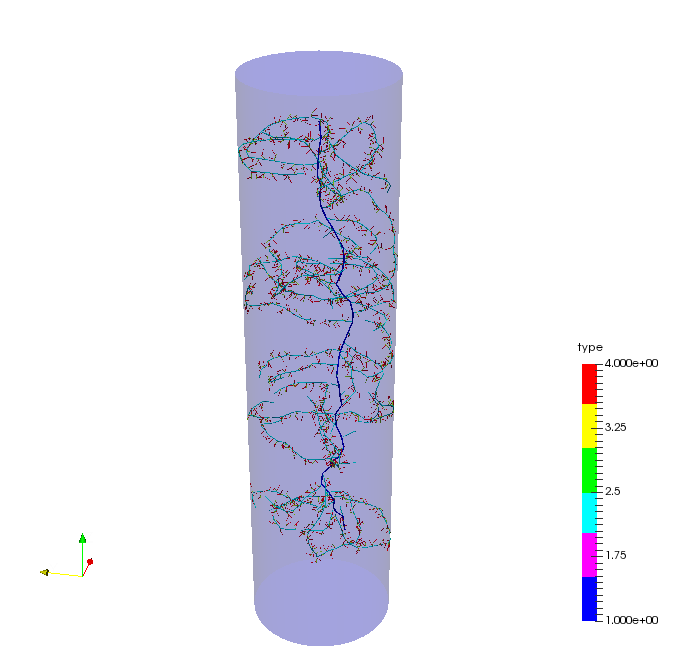
\includegraphics[width=0.99\textwidth]{example_1b.png}
\subcaption{Confined to soilcore (Example 1b)} \label{fig:basicB}
\end{subfigure}
\caption{Paraview visualizations of results of example 1a and 1b.} 
\end{figure}

Next, we show how to build more complex container geometries using SDF, 
furthermore, we show an example with multiple root systems that is computed in parallel.

\subsection{Using SDF with set operations}

In the following example we create geometries that we might encounter in experiments. 
First, we show how to rotate a rhizotron (e.g. to see more roots at the wall due to gravitropism). 
Second, we create a split box experiment, and furthermore, an example where rhizotubes act as obstacles.

The following examples demonstrates how to build a complex geometry using rotations, translations and set operations on the SDF.

\lstinputlisting[language=Python, caption=Example 1c]{../../examples/python/example1c_complexcontainer.py}

\begin{itemize}

\item[15-21] Definition of a rotated rhizotron, see Figure \ref{fig:rhizo}: 
L17 creates the flat container with a small height, this container is then rotated and translated into the desired position. 
L18 is the position where the origin will lie, and L19 the rotational matrix around the x-axis. 
In L20 the origin position is rotated. Finally, in L21 the new rotated and translated geometry is created. 
\item[23-32] Definition of of a split box, see Figure \ref{fig:split}: 
The split box is composed of a left box, a right box, and a top box connecting left and right. 
In L31 the geometry is defined by the set operation union of the three compartments. 
\item[34-49] Definition of rhizotubes as obstacles, see Figure \ref{fig:rhizotubes}: L35 is the surrounding box, 
L36 a single rhizotube, that is rotated around the y-axis in L37. 
L39-L46 create a list of rhizotubes at different locations that mimics the experimental setup. 
L48 and L49 compose the final geometry by to set operation, first a union of all tubes, 
and then cut them out the surrounding box by taking the difference. 
\item[52] Pick one of the three geometries for your simulation.
\item[62] Also more complex geometries can be visualized by the Paraview script, 
however, set operations are not really performed, only the involved geometries are visualized.
\item[65] As before we cannot visualize the container geometry in the interactive rendering, but only the roots. 

\end{itemize}

\begin{figure}
\begin{subfigure}[c]{0.3\textwidth}
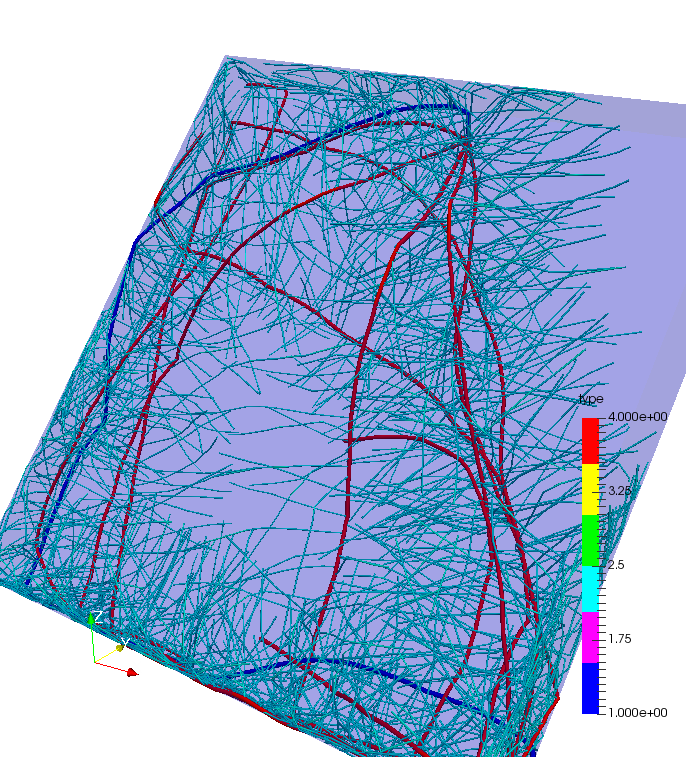
\includegraphics[width=0.99\textwidth]{example_2a1.png}
\subcaption{Rotated rhizotron} \label{fig:rhizo}
\end{subfigure}
\begin{subfigure}[c]{0.3\textwidth}
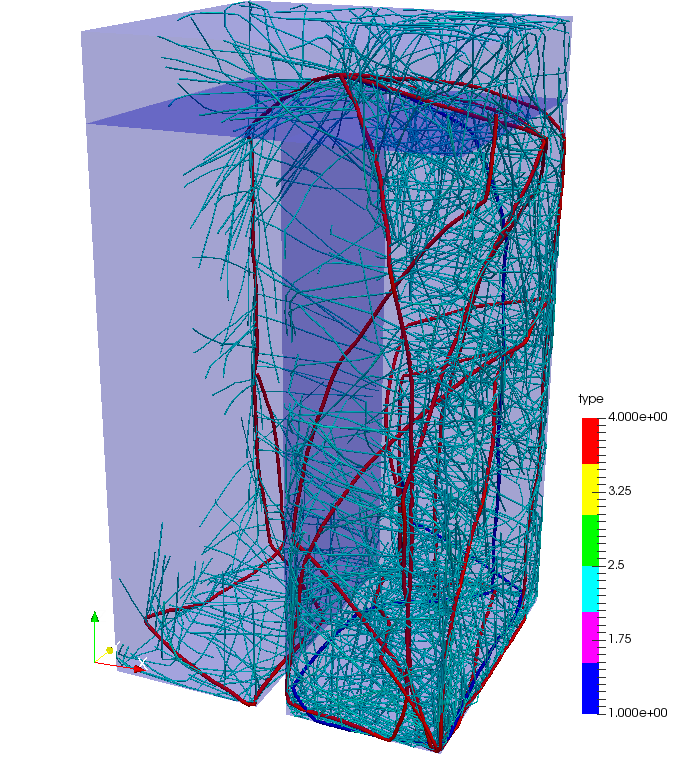
\includegraphics[width=0.99\textwidth]{example_2a2.png}
\subcaption{Split box} \label{fig:split}
\end{subfigure}
\begin{subfigure}[c]{0.3\textwidth}
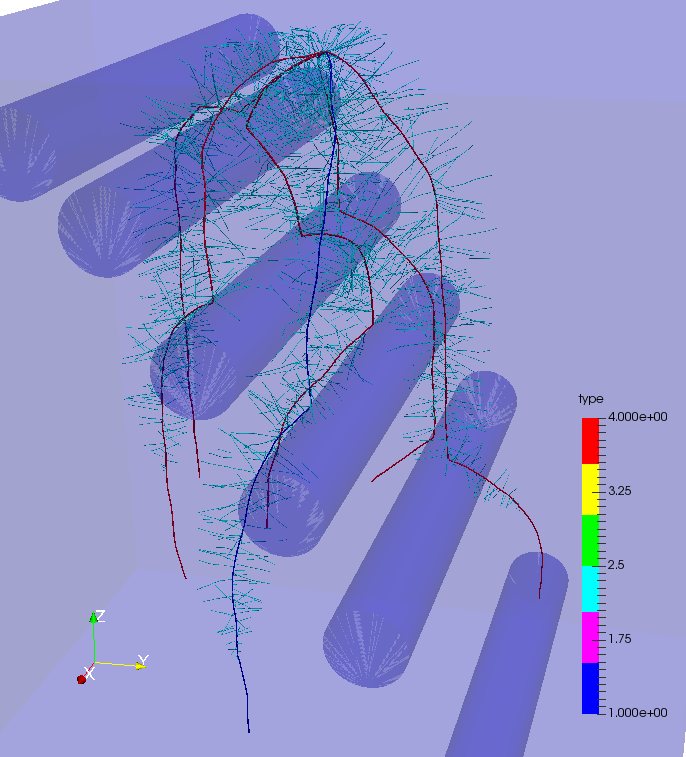
\includegraphics[width=0.99\textwidth]{example_2a3.png}
\subcaption{Rhizotubes} \label{fig:rhizotubes}
\end{subfigure}
\caption{Different geometries described by SDF (Example 1c)}
\end{figure}

\subsection{Multiple root systems}

Its possible to simulate multiple root systems. In the following we show a small plot scale simulation.

\lstinputlisting[language=Python, caption=Example 1d]{../../examples/python/example1d_multiple.py}

\begin{itemize}

\item[11,12] Set the number of columns and rows of the plot, and the distance between the root systems.

\item[15-22] Creates the root systems, and puts them into a list allRS. L20 sets the position of the seed. 

\item[25,26] Simulate all root systems 

\item[29-36] Saves each root systems, and additionally, saves all root systems into a single file. 
Therefore, we create an SegmentAnalyser (see Section \ref{sec:sa}) object in L29 and merge all segments into it L33, 
and finally export the single file L36. The resulting geometry is shown in Figure \ref{fig:multiple}.

\end{itemize}

\begin{figure}
\centering
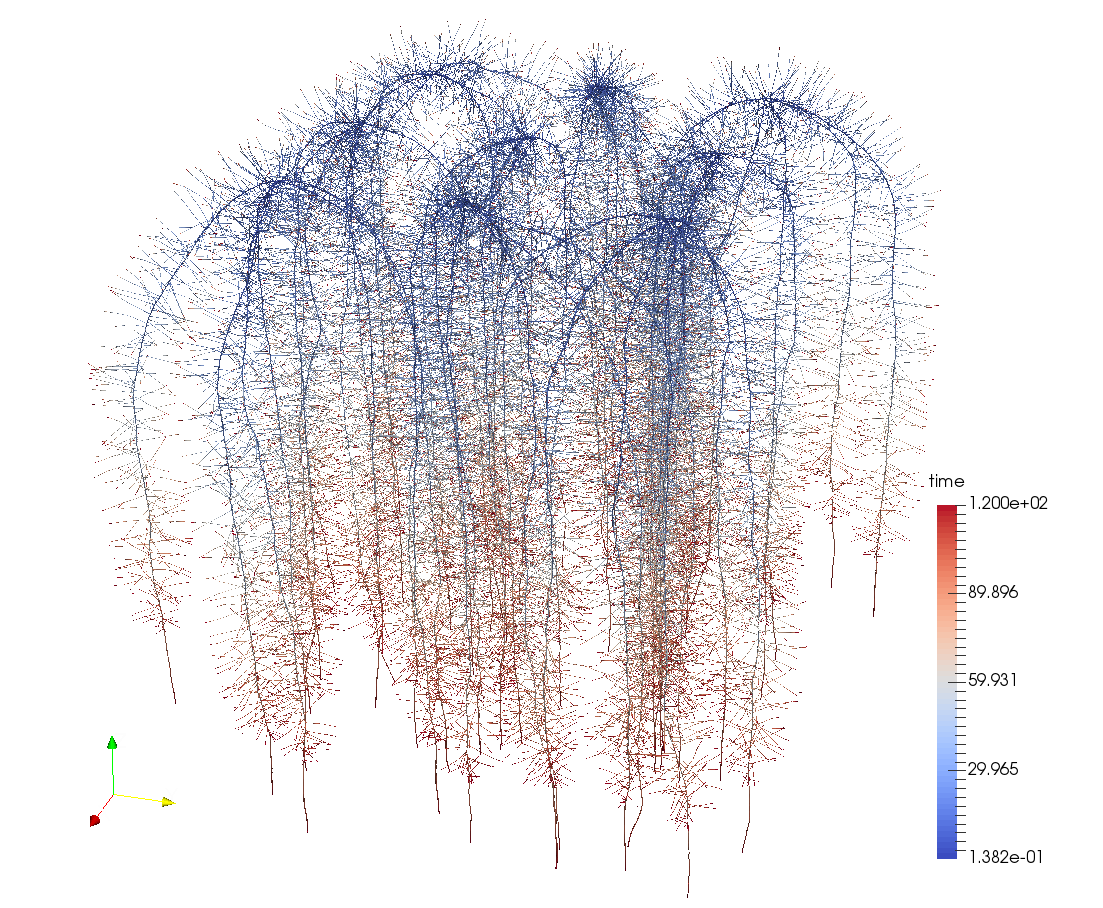
\includegraphics[width=0.7\textwidth]{example_2b.png}
\caption{Multiple root systems (Example 1d), colors denote the creation time of the root segments} \label{fig:multiple}
\end{figure}





\section{The RootSystem class} \label{sec:rs}

The class RootSystem is responsible for the model parameter and controls the simulation.
Additionally, the class offers utility functions for post processing on a per root level. 
Post processing functions per segment can be found in the class SegmentAnalyser (see Section \ref{sec:sa}).

\subsection{Initialize parameters from scratch} \label{sec:from_scratch}
 
In the previous examples we always opened the root system parameters from a file. 
In this example we show how to do everything in a Python script without the need of any parameter files. 
This is especially important if we want to modify any of the parameters in our scripts, 
like it is needed for a sensitivity analysis in Section \ref{ssec:sensitivity}.

In order to set up a simulation by hand, we have to define all relevant model parameters. 
This is done by creating a RootRandomParameter object for each root type, and 
SeedRandomParameter for each plant type. 

Note that within the simulation, the parameters for a specific root (RootSpecificParameter) 
are generated from the RootRandomParameter that represents the random distributions of certain parameters.

\lstinputlisting[language=Python, caption=Example 2a]{../../examples/python/example2a_initialize.py}

\begin{itemize}

\item[11,12] Create the root type parameters of type 1 and type 2.
\item[16-36] We set up a simple root system by hand. 
First we define the tap root L14-L27, then the laterals L29-L36. By default all standard deviations are 0. 
Most parameters standard deviations can be set with an additional 's' appended to the parameter name, 
e.g. las is the std of la, see L32
\item[38,39] Set the root type parameters.

\item[32-46] Create the seed random parameter stating when basal and shoot borne roots emerge. 
In this example we neglect shoot borne roots, and just define the seed location and  the emergence times (in days) 
of the basal roots.
\item[47] Sets the root system parameters.

\item[49] We state the root types of basal and shoot borne roots. 
Per default these types are 4 (for basal) and 5 (for shootborne). 
If they are not set a warning is produced and the tap root type 1 is taken. 
\item[50,51] Simulate and export results. 

\item[57-55] It is not only possible to set all model parameter, 
but to retrieve all parameters after the simulation with rs.getParameter. 
For all parameters that are derived from a distribution the root specific parameters are returned (L56), 
i.e. the values that were drawn from the normal distribution. 
The root random parameter can be accessed by adding '\_mean', '\_dev' to the parameter value (L57).  

\item[56-63] Simulation results can also accessed with getParameter(), 
which returns the parameter value per root. Especially, note the difference between la, and la\_mean

\end{itemize}

Note that all parameters can be set and modified within Python. 
Especially, standard deviations can be set to zero in order to be able to precisely predict the result. 
For example we can calculate the total root system length analytically, 
and check if the numerical simulation yield the (exact) same result. 
This is performed in the tests withing test\_root.py, and test\_rootsystem, 
which is used to test and validate CPlantBox and formerly CRootBox.



\subsection{Root system length over time}

The following script shows how to analyse root system length versus time. 

\lstinputlisting[language=Python, caption=Example 3a]{../../examples/python/example2b_length.py}

\begin{itemize}

\item[6] NumPy is Python's scientific computing package.
\item[7] Matplotlib is Python's easy way to create figures like in Matlab.

\item[9-14] Sets up the simulation.

\item[16-18] Defines the simulation time, time step, and the resulting number of simulate(dt) calls. 

\item[21] First we state which scalar type we want to analyse (others are type, radius, order, time, surface, one, parenttype)

\item[22] Pre-definition of the NumPy arrays storing the lengths over time. 

\item[23-30] The simulation loops executes the simulation for a single time step L24. L25 calculates the type of each root, L26 the length (or other scalar type) of the root. L27-L30 calculates the total root length in the time step for all roots, and for specific root types.

\item[32-38] Creates Figure \ref{fig:length}.

\end{itemize}



\subsection{Root tips and root bases}

Next we show two options how to retrieve root tip postions and root base positions from a simulation:

\lstinputlisting[language=Python, caption=Example 3b]{../../examples/python/example2c_roottips.py}

\begin{itemize}

\item[14,15] Reset the simulation and simulate for only 7 days (otherwise there are so many root tips).

\item[17-18] Outputs the number of nodes and segments to get an idea how big the resulting root system is. 
Note that number of segments equals the number of nodes minus the number of base roots that will emerge. 
Base roots are tap roots, basal roots and shootborne roots.

\item[20-36] The first approach retrieves all roots as polylines L50. 
Root tips are the last nodes of the polylines L54, root bases the first nodes L53. 
Roots that have not started to grow have only 1 node, and are not retrieved by getPolylines().

\item[28-31] Second approach: L29 rs.getNodes() returns all nodes of the root system as a list of Vector3d objects. 
Each Vector3d object can be converted into a numpy array automatically, 
but is necessary to do that for each element of the list. The methods L30, L31 return the indices of the tips and bases. 

\item[33-41] Creates Figure \ref{fig:scatter} using the second approach.

\item[44,45] Verifies that both approaches yield the same result.

\end{itemize}

\begin{figure}
\begin{subfigure}[c]{0.5\textwidth}
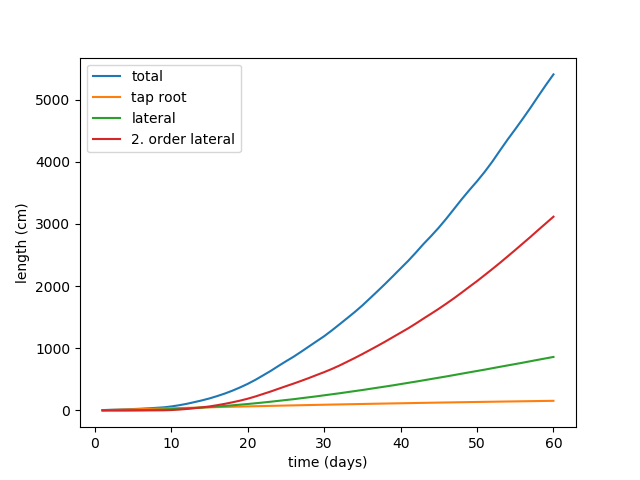
\includegraphics[width=0.99\textwidth]{example_3a.png}
\subcaption{Total root length versus time} \label{fig:length}
\end{subfigure}
\begin{subfigure}[c]{0.5\textwidth}
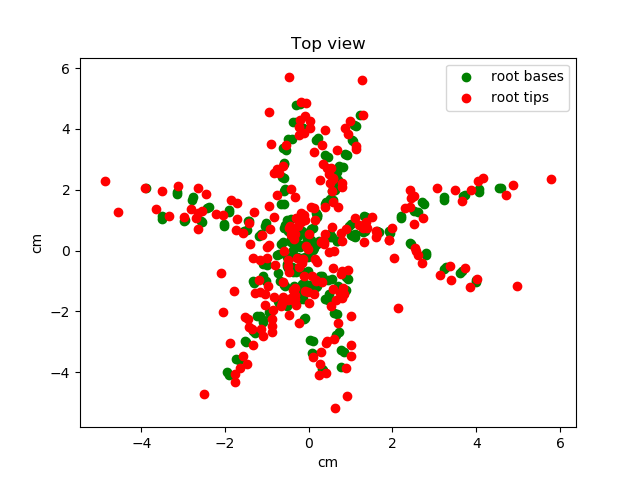
\includegraphics[width=0.99\textwidth]{example_3b.png}
\subcaption{Top view of the root tip and root bases} \label{fig:scatter}
\end{subfigure}
\caption{Root system analysis: Example 2b (a), Example 2c (b)} 
\end{figure}




% \subsection{Analysis per segment, rootsystem length density}
% 
% The class SegmentAnalyser offers post-processing methods per root segment. The advantage is that we can do distributions or densities, and that we can crop the segments with any geometry. 
% 
% We start with a small example plotting the root surface densities of a root system versus root depth.
% 
% \lstinputlisting[language=Python, caption=Example 3c]{../../examples/python/example3c.py}
% 
% \begin{figure}
% \centering
% 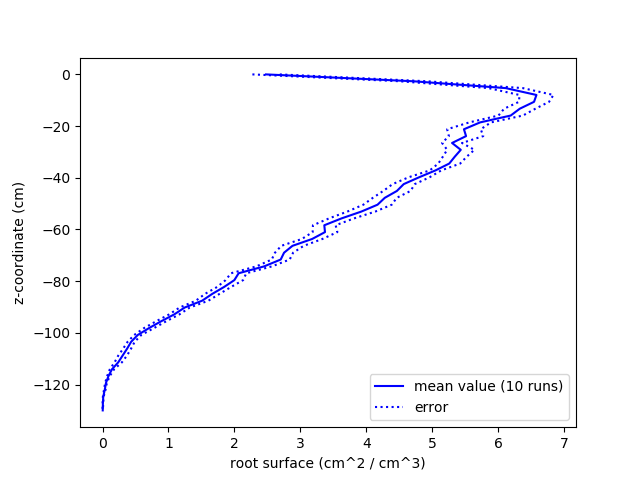
\includegraphics[width=0.7\textwidth]{example_3c.png}
% \caption{Root surface densitiy versus depth mean (Example 3c), and standard error ($N$=10)} \label{fig:surface_density}
% \end{figure}
% 
% 
% \begin{itemize}
% 
% \item[8-12] Pick a root system.
% \item[14-16] Depth describes the y-axis of the graph, layers the number of vertical soil layers, where the root surface is accumulated, and runs is the number of simulation runs. 
% \item[18-23] Perfoms the simulations. L23 creates a distribution of a parameter (name) over a vertical range (bot, top). The data are accumulated layers, segments are either cut (exact = True) or accumaled by their mid point (exact = False). 
% \item[25] In order to calculate a root surface density from the summed up surface, we need to define a soil volume. The vertical height is the layer length, lenght and widht (here 10 cm), can be determined by planting widht, or by geometry, if root growth is confined. 
% \item[26-28] Calculates the densitis, mean densities, and standard error. 
% \item[30-39] Prepares teh plot (see Figure \ref{fig:surface_density}).
% 
% \end{itemize}
% 
% 
% 
% \subsection{Analysis per segment using SDF}
% 
% The following script demonstrates some of the post processing possibilities by setting up a virtual soil core experiment, where we analyse the content of two soil cores located at other positions.
% 
% \lstinputlisting[language=Python, caption=Example 3d]{../../examples/python/example3d.py}
% 
% \begin{itemize}
% 
% \item[9-15] Performs the simulation.
% 
% \item[17-20] We define two soil cores, one in the center of the root and one 10 cm translated. In L16 we pick which one we use for the further analysis.  Figure \ref{fig:soilcoreGeom} shows the resulting geometry.
% 
% \item[23] We pick which geometry we will use for further analysis.
% 
% \item[25-29] Prepares the plot. We use four sub-figures. 
% 
% \item[31-35] Creates a root length distribution versus depth. L32 creates the SegmentAnalyser object, and L41 creates the distribution.
% 
% \item[37-43] Performs the same distribution in the soil core. In L39 we crop the segments to the geometry. L49 is used to delete unused nodes. 
% 
% \item[45-52] Same as before, but we are only interested in segments that are younger than 30 days. In L47 we use the filer method (name, min, max) to keep only the segments we want in the analysis. 
% 
% \item[54-61] The filter method can be used for many different applications. In the following we use it to analyse lateral roots only. Possible rb.ScalarType are: 'type', 'radius', 'order', segment creation time 'time', 'length', 'surface', 'volume', 'one', 'userdata1', 'userdata2', 'userdata3', and 'parenttype'.
% 
% \item[63-65] Show and save resulting Figure \ref{fig:central}, and \ref{fig:shifted}.
% 
% \end{itemize}
% 
% In this example the central core captures only a little amount of laterals (Figure \ref{fig:central}) because the root system is wide spread. 
% The shifted root core represents the overall root system slightly better, see Figure \ref{fig:shifted}.  
% The basic idea is that such simulations help to increase the understanding of experimental observations.
% 
% \begin{figure}
% \centering
% 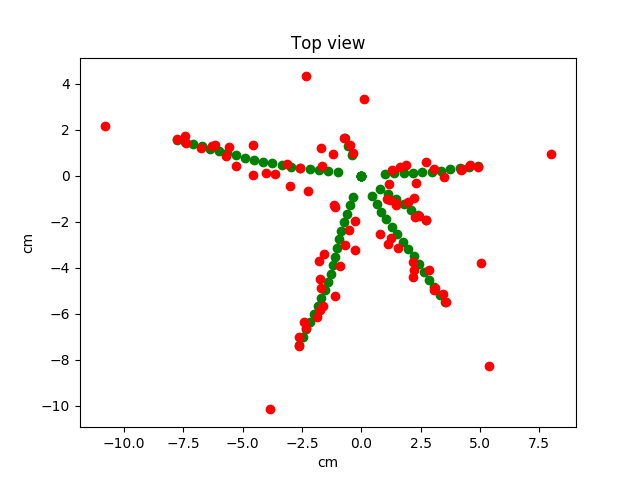
\includegraphics[width=0.7\textwidth]{example_3d.png} % 
% \caption{Virtual soil cores experiment (Example 3d): Central core (blue), shifted core (red)} \label{fig:soilcoreGeom}
% \end{figure} 
% 
% \begin{figure}
% \centering
% 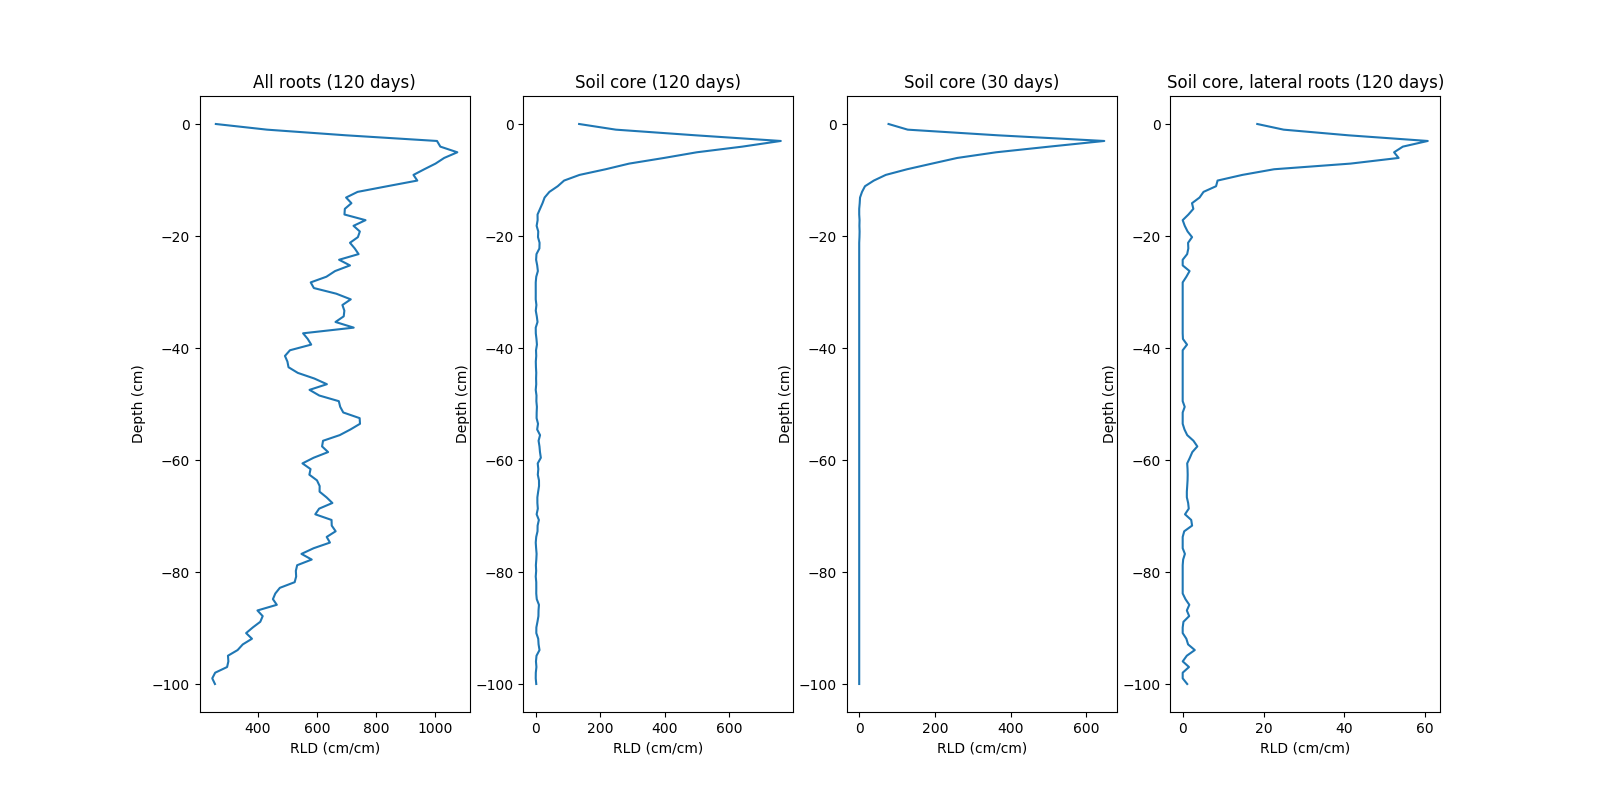
\includegraphics[width=0.9\textwidth]{example_3d1.png} 
% \caption{Central core (Example 3d)} \label{fig:central}
% \end{figure}
% 
% \begin{figure}
% \centering
% 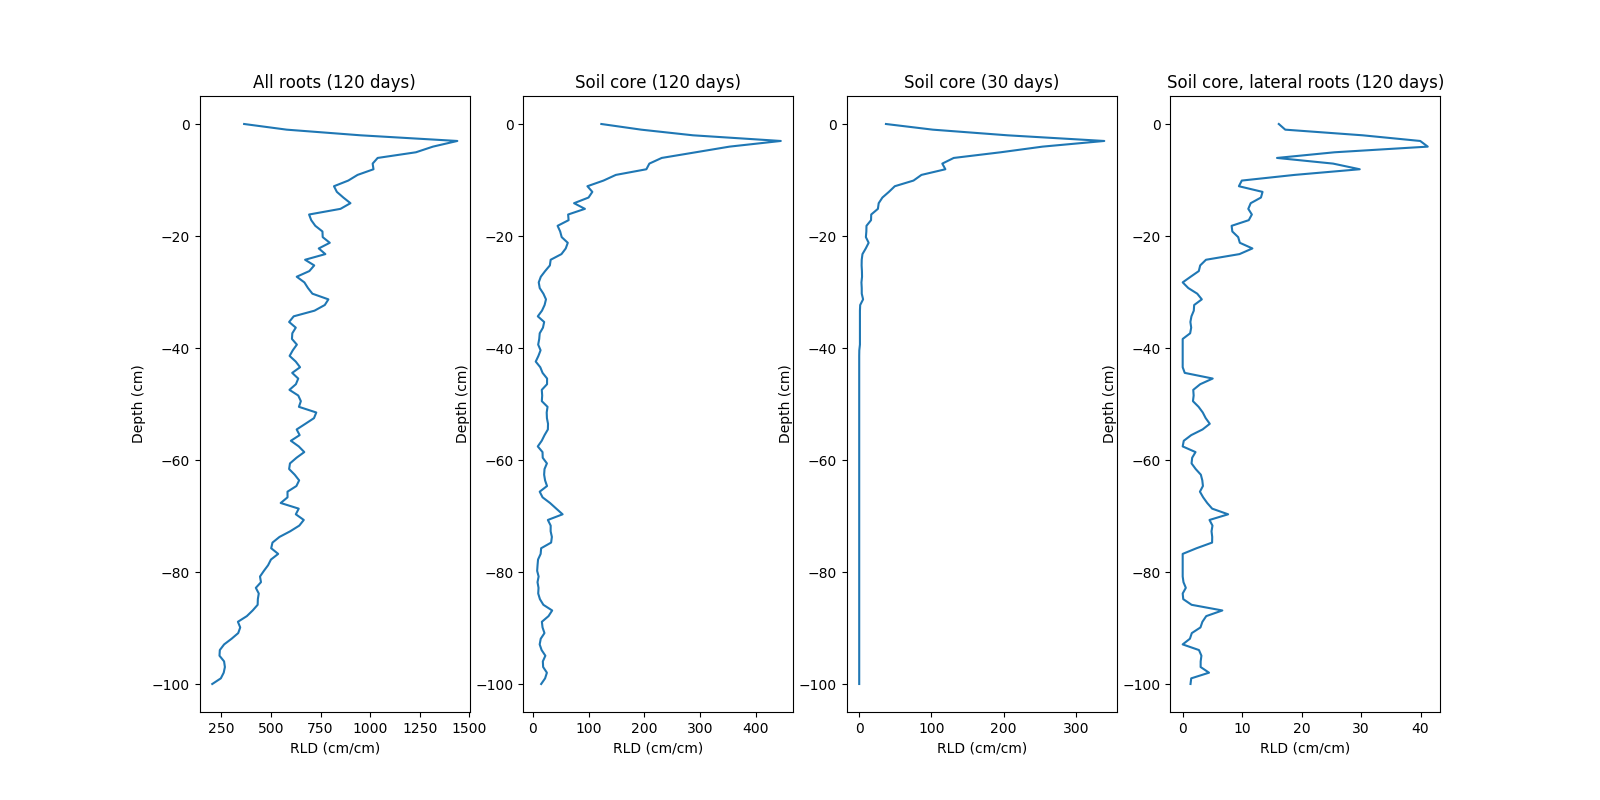
\includegraphics[width=0.9\textwidth]{example_3d2.png} 
% \caption{Shifted core (Example 3d)} \label{fig:shifted}
% \end{figure}
% 
% 
% \subsection{SegmentAnalyser for DGF or VTP export}
% 
% If we want to export our root system as dune grid file (dgf) we need to introduce an artificial shoot. By default the tap root and basal root starts at the seed node (i.e. multiple segments start at the same node), and its difficult to define a boundary condition in Dumux for such a situation. Furthermore, if there are shoot borne roots, they emerge out of nothing above the seed node. Therefore, we introduce artifical segments eventually connecting shoot borne roots (if there are any) and connecting the seed node (noramlly located at 0,0,-3) to the orgin at (0,0,0). The following code snippet shows how to export a RootSytem dgf:
% 
% \lstinputlisting[language=Python, caption=Example 3e]{../../examples/python/example3e.py}
% 
% \begin{itemize}
%  \item[6-11] Define a example root sytemytem
%  \item[13] Create the analyser object
%  \item[15-18] Get the artificial shoot segments from the root sytem (L15) and manually add them ot the SegmentAnalyser (L18).
%  \item[20] Write the DGF file 
% \end{itemize}
% 
% It is also possible to make use of the SegmentAnalyser class without any ohter CPlantBox classes (e.g. for writing vtp from measurements). The following example shows how to construct the class with arbitrary nodes and segments (e.g. from measurements). 
% 
% \lstinputlisting[language=Python, caption=Example 3f]{../../examples/python/example3f.py}
% 
% \begin{itemize}
%  \item[6-9] Define some segments with data
%  \item[14,15] We convert the Python list to lists of C++ types
%  \item[20] We create the SegmentAnalyser object without an underlying Organsim
% \end{itemize}
% 
% 
% 
% \section{Model parameters} %Chapter 4
% 
% In the following we show how model parameters can be modified, and how a sensitivity analysis can be performed. Additionally, we comment on how to best make an animation from a CPlantBox simulation.
% 
% \subsection{Set up a simulation from 
% \subsection{Sensitivity analysis} \label{sec:sa}
% 
% In the next part we vary given parameters in order to make a sensitivity analysis. This takes a lot of simulation runs and we demonstrate the of use parallel computing to speed up execution.
% 
% In this exmemplary sensitivity analysis ww will vary the insertion angle of the tap and basal root, and look at the resulting change in mean root tip depth and radial distance. 
% 
% \lstinputlisting[language=Python, caption=Example 4b]{../../examples/python/example4b.py}
% 
% \begin{itemize}
% 
% \item[12-20] Defines a function to set all standard deviations proportional to the parameter values. We use this function in the following to set the standard deviation to zero everywhere. 
% 
% \item[23-29] Parameters of the analysis. $N$ denotes the resolution of the parameter we vary, and $runs$ the number of iterations, i.e. a total of $N\cdot runs$ simulations are performed. In L29 we define the insertion angle to be varied linearly between 0 and $\pi/2$.
% 
% \item[32-52] Definition of a function that performs the simulation and returns mean root tip depth and radial distance. First we create a root system and set the standard deviation to zero L34-L36. L38, L39 sets the insertion angle. L41 initializes the root system and states that basal root are of root tape 1 (same as tap root). The False value turns of verbosity to avoid any outputs to the console. L42 performs the simulation. L44-L52 calculates the mean root tip depth and radial distance. 
% 
% \item[55-73] This section performs the computation of all simulation runs. L55-56 preallocates the resulting arrays. L62-L68 performs the parallel computations, index $i$ is the index of the insertion angle. L71-73 calculates the mean values.
% 
% \item[75-85] Creates the resulting Figure \ref{fig:sa}
% 
% \end{itemize}
% 
% \begin{figure}
% \centering
% 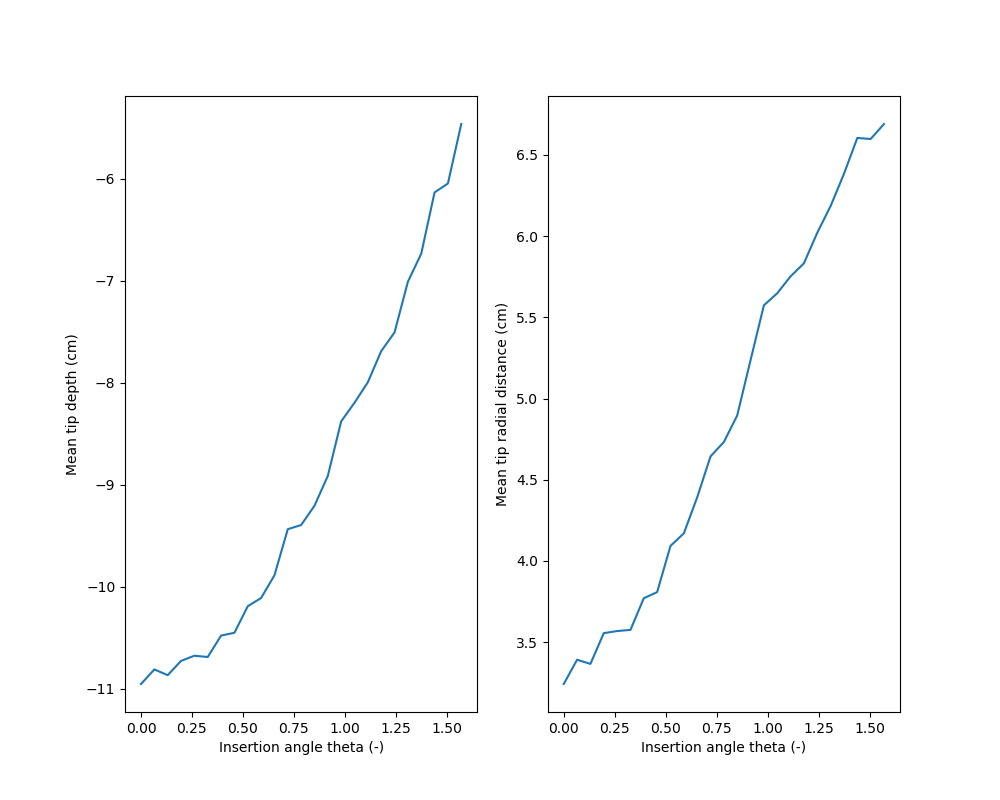
\includegraphics[width=0.7\textwidth]{example_4b.png}
% \caption{Sensitivity of mean root tip depth (left) and radial distance (right) to the insertion angle theta (Example 3d) } \label{fig:sa}
% \end{figure}
% 
% \subsection{How to make an animation}
% 
% In order to create an animation in Paraview we have to consider some details. The main idea is to export the result file as segments using the class SegmentAnalyser. A specific frame is then obtained by thresholding within Paraview using the segments creation times. 
% 
% We modify example1b.py to demonstrate how to create an animation.
% 
% \lstinputlisting[language=Python, caption=Example 4c (modified from Example 1b)]{../../examples/python/example4c.py} 
% 
% \begin{itemize}
% 
% \item[17,18] Its important to use a small resolution in order to obtain a smooth animation. L18 set the axial resolution to 0.1 cm. 
% 
% \item[25] Instead of saving the root system as polylines, we use the SegmentAnalyser to save the root system as segments.
% 
% \item[28] We save the geometry as Python script for the visualization in ParaView.
% 
% \end{itemize}
% 
% After running the script we perform the following operations to create an animation:
% \begin{enumerate}
%  \item Open the .vtp file in ParaView (File$\rightarrow$Open...), and open tutorial/examples/python/results/example\_4c.vtp.
%  \item Optionally, create a tube plot with the help of the script tutorial/pyscript/rsTubePlot.py (Tools$\rightarrow$Python Shell, press 'Run script').
%  \item Run the script tutorial/pyscript/rsAnimate.py (Tools$\rightarrow$Python Shell, press 'Run script'). The script creates the threshold filter and the animation. 
%  \item Optionally, visualize the domain boundaries by running the script tutorial/examples/python/results/example\_4c.py (Tools$\rightarrow$Python Shell, press 'Run script'). Run after the animation script (ohterwise it does not work).  
%  \item Use File$\rightarrow$Save Animation... to render and save the animation. Pick quality (<100 \%), and the frame rate in order to achieve an appropriate video length, e.g. 300 frames with 50 fps equals 6 seconds. Files might be very big, and needs compression (e.g. ffmpeg -i in.avi -vcodec libx264 -b 4000k -an out.avi, produces high quality, tiny file size, and plays with VLC).
% \end{enumerate}
% 
% 
% 
% \section{Tropisms} % chapter 5
% 
% The change in root growth direction is described by tropisms. 
% 
% 
% \subsection{Hydro- and chemotropism} \label{sec:hydro}
% 
% Root growth direction is influenced by soil conditions such as water content, soil strength, or nutrient concentration. 
% In the following we show how this is achieved in CRootBox.
% 
% \lstinputlisting[language=Python, caption=Example 5a]{../../examples/python/example5a.py}
% 
% \begin{itemize}
% 
% \item[3-5] Creates the root system and opens the parameter file
% 
% \item[7-14] Change the tropism for the first ten root types: L10 retrieves the parameter, where the CRootBox parameters run from 1 to 11. L11 modifies the axial resolution, and L12-14 sets the three tropism parameters. 
% 
% \item[16-22] Definition of a static soil property using SDF. We first define the geometry (L20-L21), and then create a static soil (L22) that obtains the maximal value $maxS$ inside the geometry, 
% $minS$ outside the geometry, and linear slope with length $slope$. At the boundary the soil has the value $(maxS+minS)/2$.
% 
% \item[25] Sets the soil. Must be called before RootSystem::initialize()
% 
% \item[28] Initializes the root system, and among others sets up the hydrotropism. 
% 
% \item[30-36] Simulation loop
% 
% \item[39] Exports the root system geometry
% 
% \item[42-43] We actually do not wish to set this geometry, but we abuse the writer of the class RootSytem to export a Python script showing the layer geometry. The resulting ParaView visualization is presented in Figure \ref{fig:chemo}.
% 
% \end{itemize}
% 
% \begin{figure}
% \centering
% 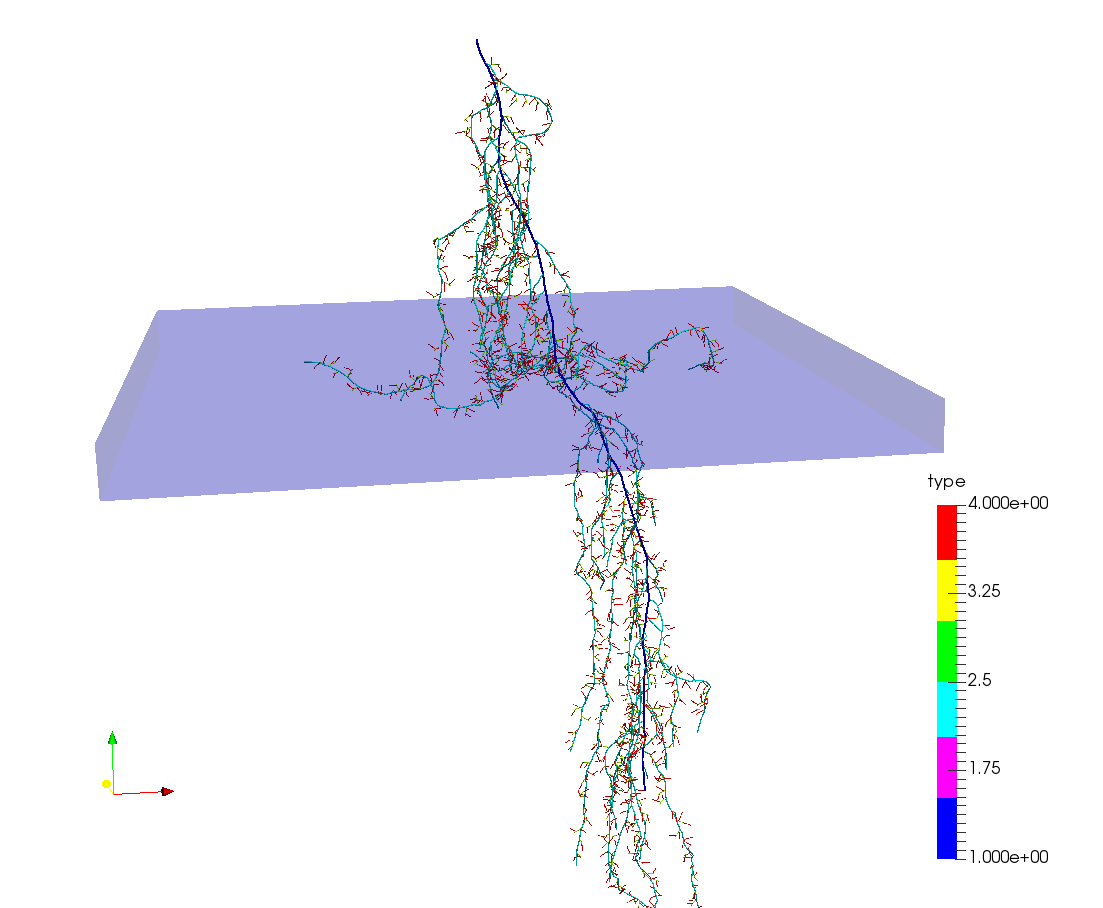
\includegraphics[width=0.7\textwidth]{example4a.png}
% \caption{Chemotropism in a nutrient rich layer (Example 4a)} \label{fig:chemo}
% \end{figure}
% 
% 
% 
% \subsection{User defined tropisms} \label{sec:usertropism}
% 
% Normally, the simulation is created from a set of parameters. For tropisms these are the type of tropism $tt$, number of trials $N$ , and tortuosity $\sigma$.
% There are two ways to add user defined tropisms: 
% 
% \begin{enumerate}
% \item The first is C++ only: It is to extend the CRootBox class and overwrite the method RootSystem::createTropism. 
% This is the function that is called, when the tropisms are created from the parameters ($tt$, $N$, $\sigma$) in RootSystem::initialize(). 
% This is necessary when user defined tropism are created from a parameter file, where $tt$ is the number of the new tropism type. 
% \item The second is to manually set the tropisms using the method RootSystem::setTropism. Make sure to call Rootsystem::setTropism($\dots$) after Rootsystem::initialize().
% \end{enumerate}
% 
% In both approaches the user has to extend the new tropism class from the class Tropism. 
% If just the objective function of the tropism is changed, it is enough to overwrite Tropism::tropismObjective. 
% This can done in Python or in C++,the classes Hydrotropism, Gravitropism, and Plagiotropism are examples for this procedure.
% 
% If the whole concept of the random optimization is altered, Tropism: :getUCHeading must be overwritten. 
% If the geometry model is also changed Tropism: :getHeading must be overwritten.
% 
% The following example shows how to implement a new tropism in Python. Two new tropism are introduced:
% The first does nothing put to output the incoming arguments of the method Tropism::tropismObjective to the command line (e.g. for debugging).  
% The second one, is a Plagiotropism that changes with time to Gravitropism depending on the root age.
% 
% \lstinputlisting[language=Python, caption=Example 5b]{../../examples/python/example5b.py}
% 
% \begin{itemize}
% 
% \item[3-14] Creates a new tropism that just writes incoming arguments of Tropism: :tropismObjective to the command line. This can be used for debugging. The new class is extended from rb.Tropism, 
% and the method Tropism::tropismObjective is overwritten with the right number of arguments.
% 
% \item[16-32] Again, we extend the new class from rb.Tropism. In L19-24 we define our own constructor.
% Doing this two things are important: (1) the constructor of the super class must be called (L20), and (2) the tropism parameters $n$, and $\sigma$ must be set (L23). 
% Furthermore, the constructor defines two tropisms: plagio- and gravitropism, that are used in Tropism::tropismObjective at a later point, and a root age, when to switch from plagi- to gravitropism. \\
% In L26-L32 the method Tropism::tropismObjective is defined. We choose the predefined objective function depending on the root age.
% 
% \item[34-38] Sets up the simulation.
% 
% \item[40-44] L40,L41 creates the first user defined tropsim. Since we did not define a constructor Tropism::setTropismParameter must be called. L43 creates the second user defined tropism. 
% In L44 the tropism is chosen, using the method Tropism::setTropism. The second argument states for which root type it applies. 
% Number 2 is the root type number of the laterals, -1 states that the tropism applies for all root types (default = -1).
% 
% \item[46-51] The simulation loop. 
% 
% \item [54] Exports the result producing Figure (\ref{fig:tropism}). Comparing to Figure (\ref{fig:basicA}) we can see the effect of the new user defined tropsim.
% 
% \end{itemize}
% 
% \begin{figure}
% \centering
% 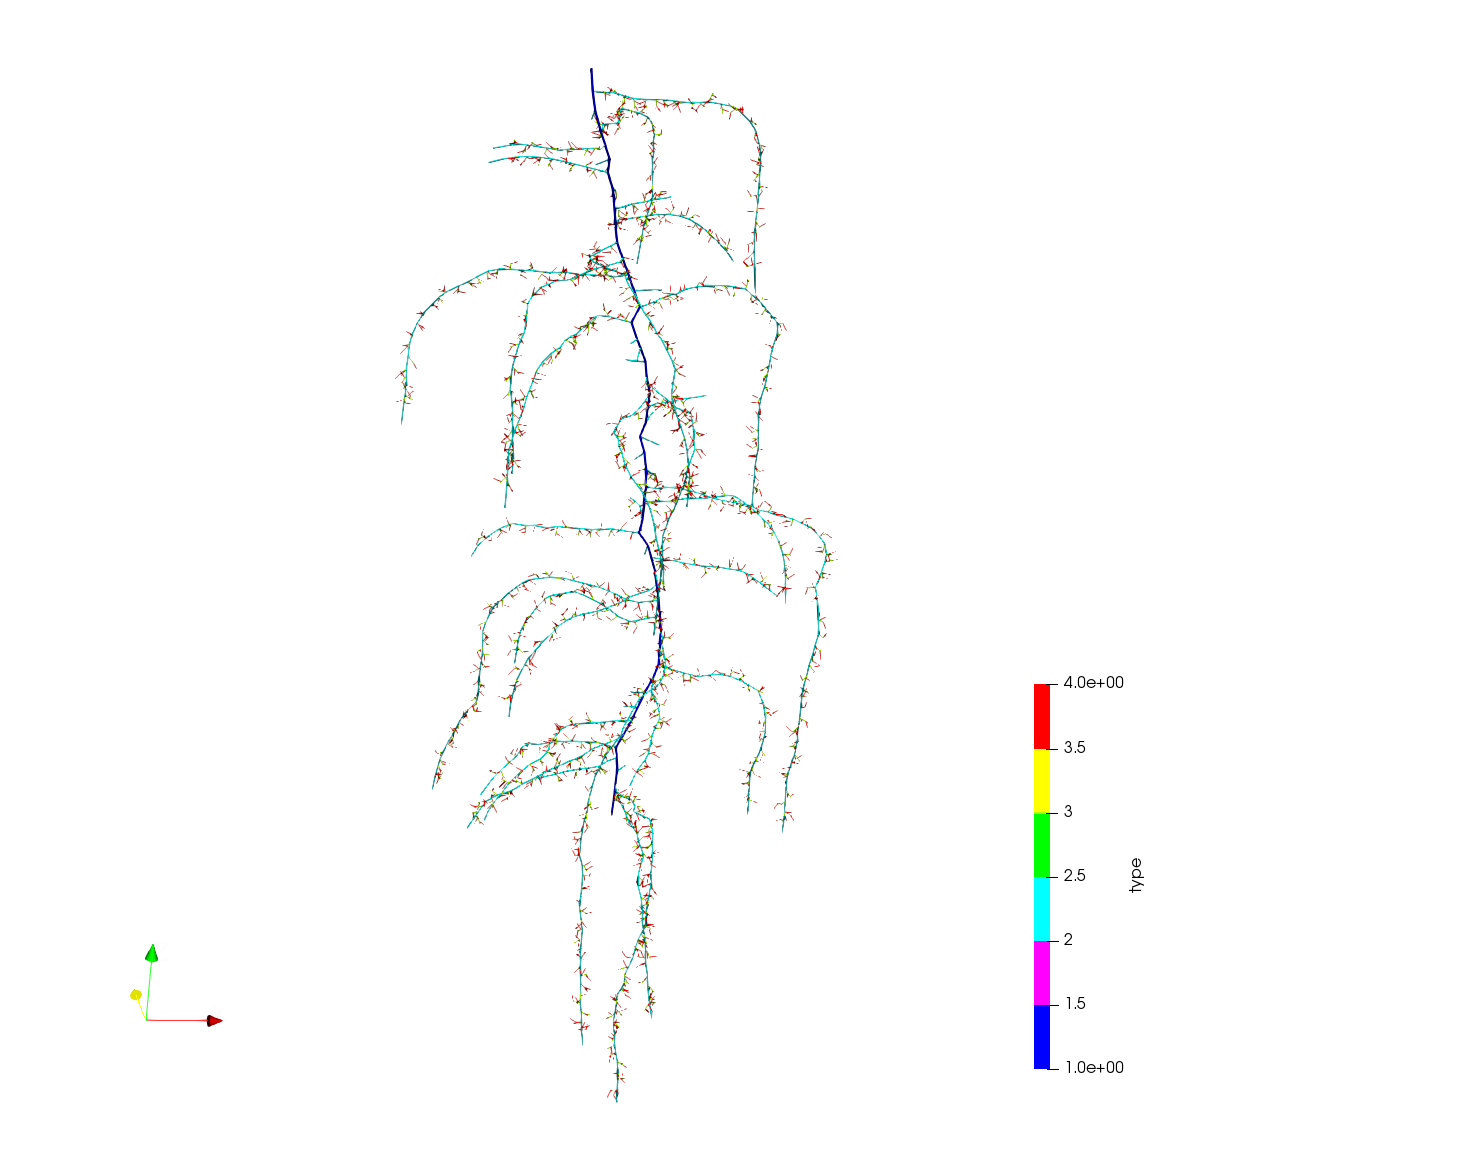
\includegraphics[width=0.7\textwidth]{example4b.png}
% \caption{Depending on root age the laterals follow plagio- or gravitropism (Example 4b)} \label{fig:tropism}
% \end{figure}
% 
% 
% 
% \section{Root functional modelling}
% 
% Root growth is strongly influenced by pedo-climate conditions, and plant internal state. CRootBox offers build in ways to develop such models. 
% In this section we assume static soil conditions, and describe predefined ways how the soil can affect root growth.
% Dynamic soil conditions are described in the following section 'Coupling with a soil model'. 
% 
% Implemented root responses are (1) the change in direction of the growing root tip, described in Sections \ref{sec:hydro} and \ref{sec:usertropism} 
% (2) the scaling of the elongation rate (3) the change of insertion angle (4) the change of lateral emergence probability, (2)-(4) are described in Section \ref{sec:elongation}.
% 
% \subsection{Scaling elongation rate, insertion angle, and lateral emergence probability} \label{sec:elongation}
% 
% The following script is an example to this and the following two sections, where (a) the elongation rate, (b) the insertion angle, and (c) the probability of lateral emergence are scaled.
% 
% Without giving a specific model these mechanisms are considered important. 
% For example the elongation rate as well as the probability of lateral emergence is dependent on soil properties like water saturation, soil strength, and temperature (among others).  
% The insertion angle is reported to be dependent on nutrient supply in some species. Furthermore, theses mechanisms are influenced by plant systemic responses.
% 
% The scaling itself can be performed in the following way:
% 
% \lstinputlisting[firstline=1,lastline=50, language=Python, caption=Example 6a (1)]{../../examples/python/example6a.py}
% 
% \begin{itemize}
% 
% \item[4-6] Creates the root system and opens the parameter file
% 
% \item[8-13] We create a confining box with two overlapping boxes left and right. This geometries are used for later analysis.
% 
% \item[15-21] We define two static soil properties using SDF (L20, L21) as explained in Section \ref{sec:hydro}. 
% The left compartment has the value $minS$, the right $maxS$, between them is a linear gradient of length $slope$.
% 
% \item[23-34] Sets the scaling functions. L24-L28 adjusts axial resolution and tortuosity $sigma$. L31 sets the scale elongation function $se$ to the soil property. L34 sets the scale insertion angle function $sa$. 
% Comment and uncomment the relevant code parts to achieve the desired scaling, to achieve the resulting Figures \ref{fig:elongation} and \ref{fig:insertion}.
% 
% \item[36-41] Sets the lateral emergence probability. 
% First, we increase the number of laterals of the first laterals (root type 2) by a factor of five and decrease the inter-nodal distances for the same factor L37-L39. This is the maximal lateral density that can be achieved.
% Then, we set the scale branching probability function $sbp$ to the soil property defined in L21, see Figure \ref{fig:probability}.
% 
% \item[44-49] Initialization and simulation loop.
% 
% \end{itemize}
% 
% \begin{figure}
% \begin{subfigure}[c]{0.3\textwidth}
% 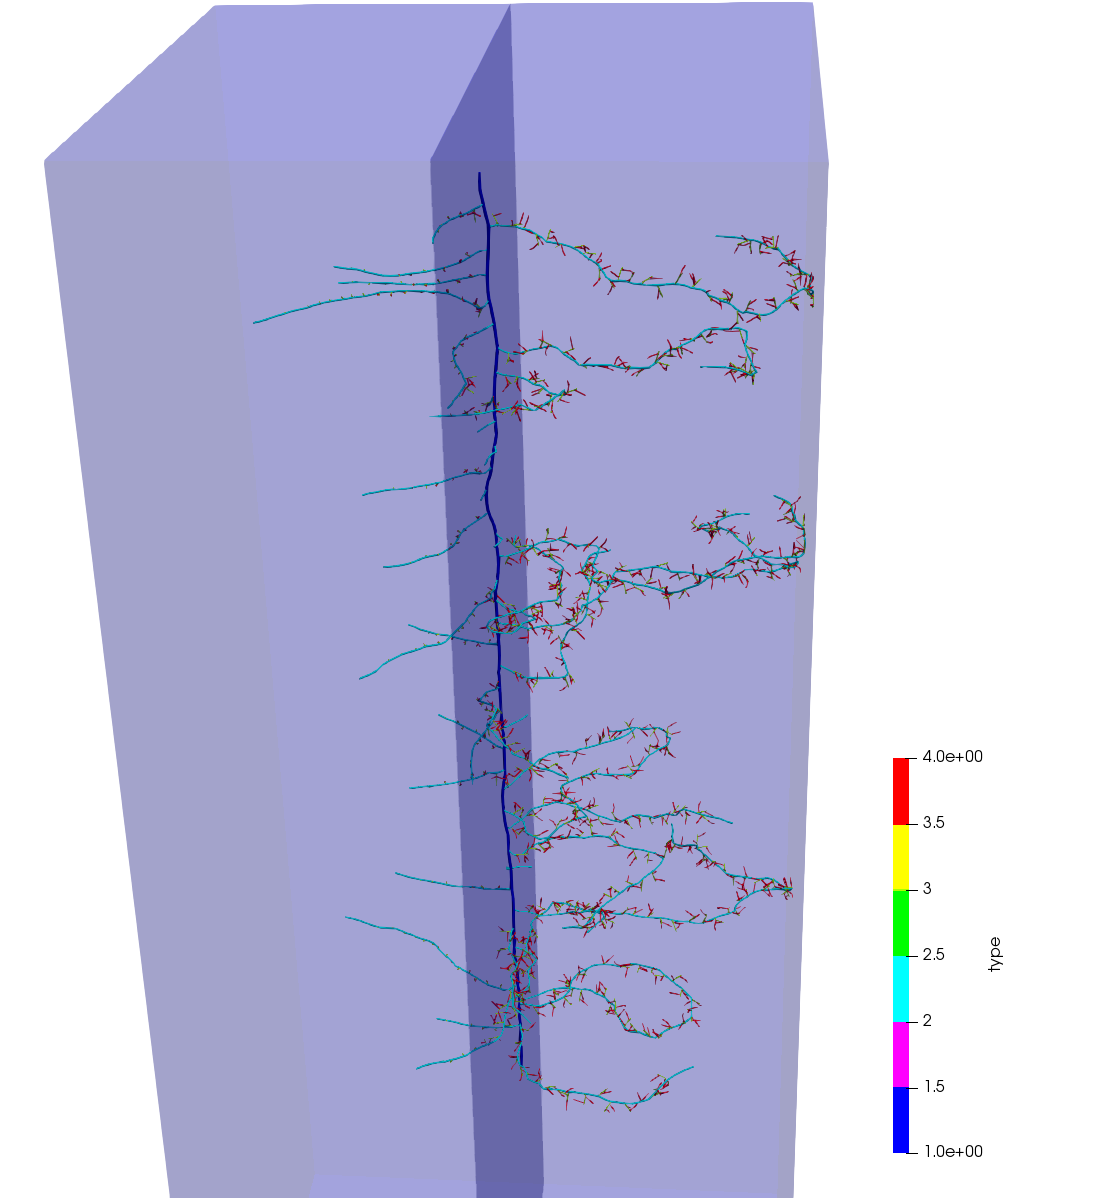
\includegraphics[width=0.99\textwidth]{example4c1.png}
% \subcaption{Root elongation rate} \label{fig:elongation}
% \end{subfigure}
% \begin{subfigure}[c]{0.3\textwidth}
% 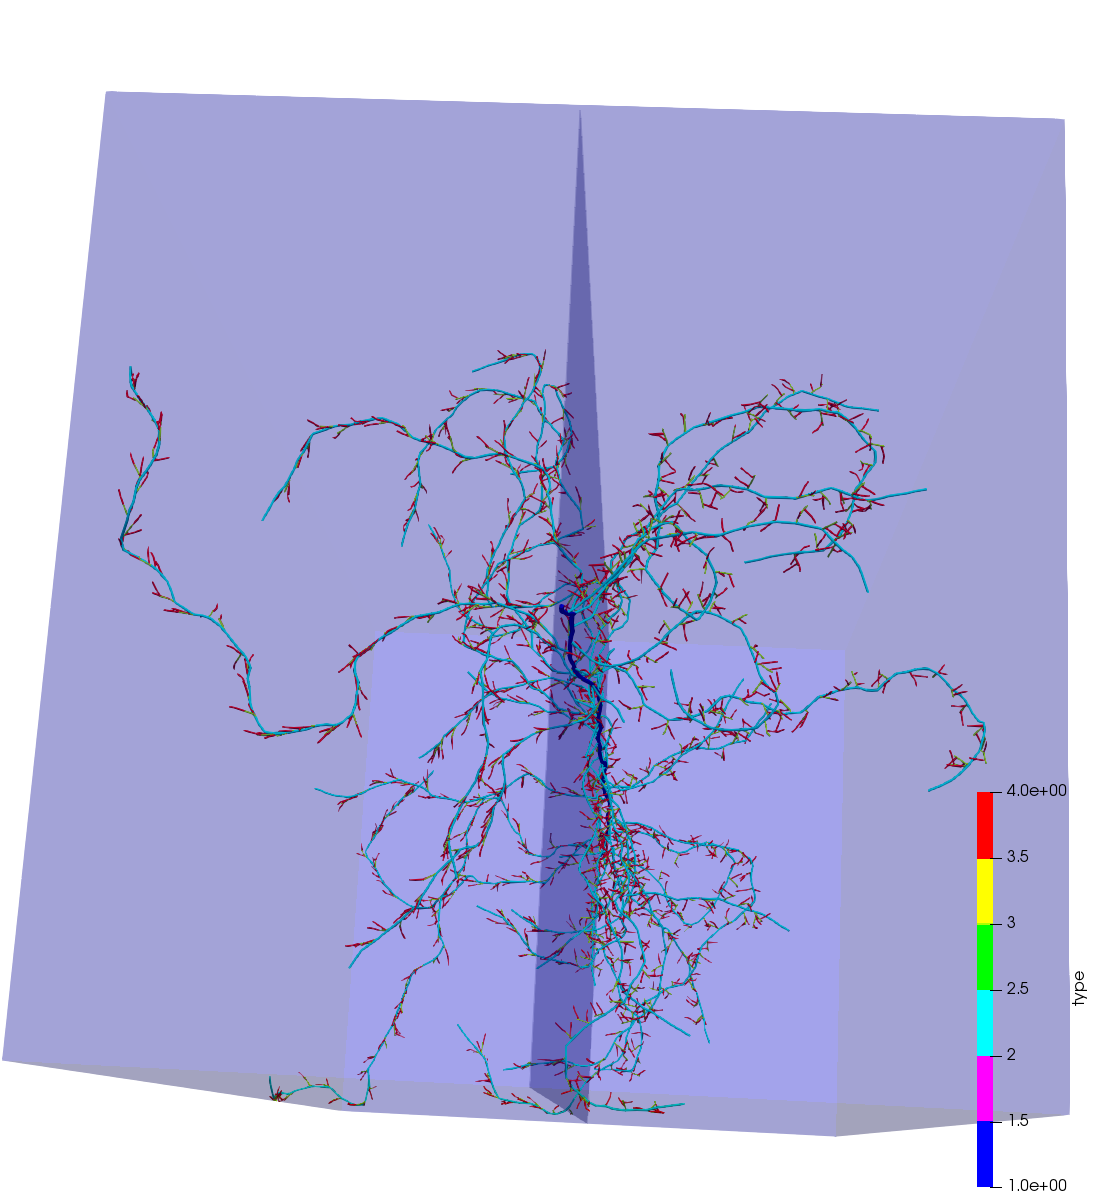
\includegraphics[width=0.99\textwidth]{example4c2.png}
% \subcaption{Insertion angle of laterals} \label{fig:insertion}
% \end{subfigure}
% \begin{subfigure}[c]{0.3\textwidth}
% 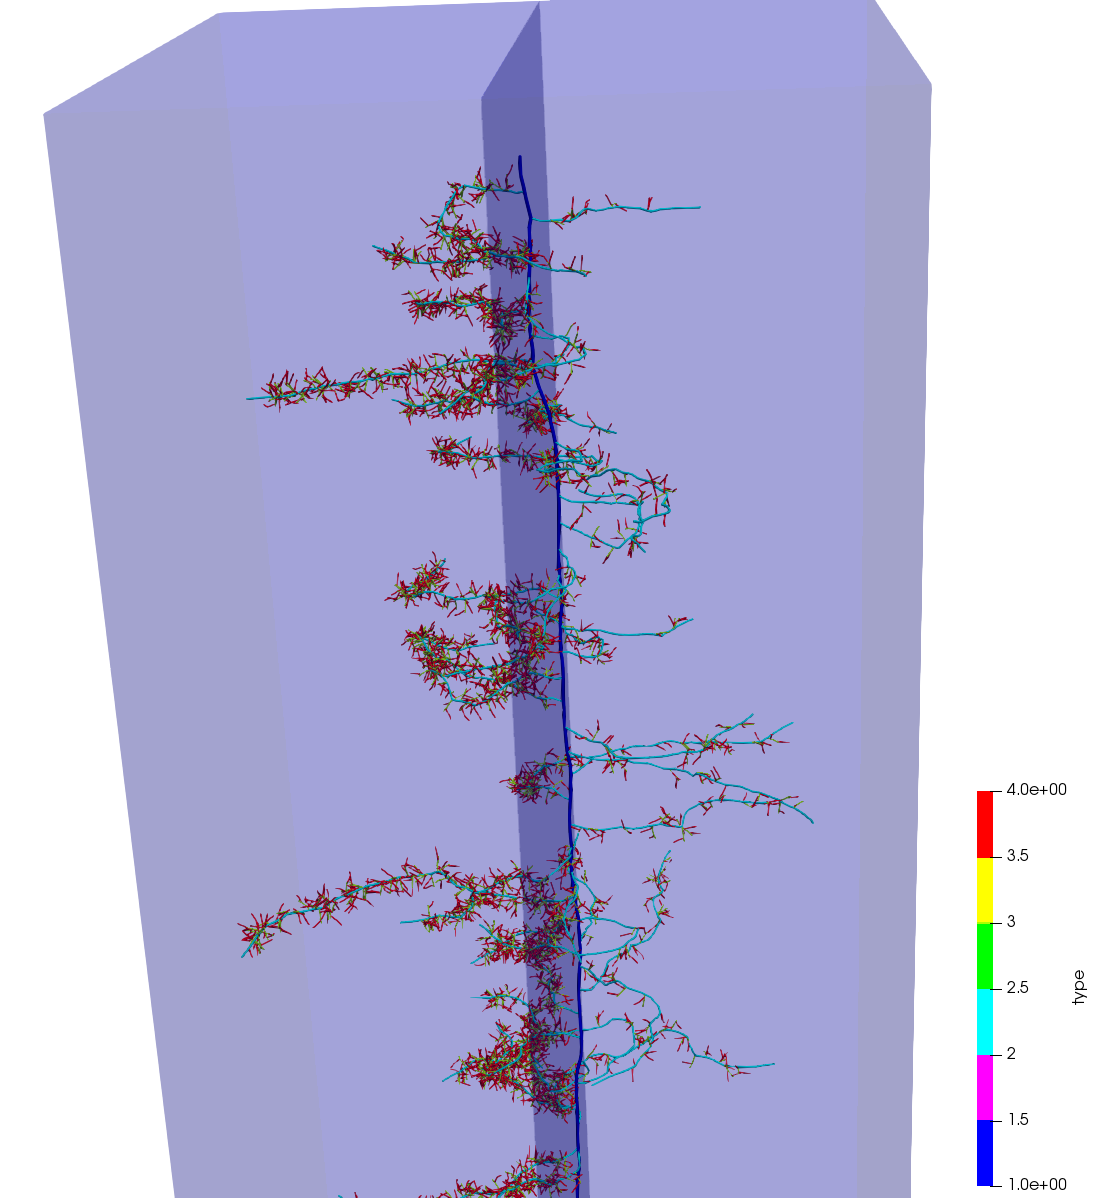
\includegraphics[width=0.99\textwidth]{example4c3.png}
% \subcaption{Branching density (probabilistic model)} \label{fig:probability}
% \end{subfigure}
% \caption{Predefined root responses (Example 4c)}
% \end{figure}
% 
% When playing with model parameters, it is not always clear if the suggested effect is realized from the figures alone. The following script helps to quantify the effects of above simulation: 
% 
% \lstinputlisting[firstline=51,lastline=81, language=Python, caption=Example 6b´ (2)]{../../examples/python/example6b.py}
% 
% 
% \subsection{Soil} \label{sec:soil}
% 
% 
% \subsection{User defined soil} \label{sec:usersoil}
% 
% 
% 
% 
% \section{Model coupling}
% 
% In the previous section root responses were described in a static soil. 
% In this section we will extend this to a dynamic soil setting, where we update the soil in the simulation loop, and then update the root system iteratively for small time steps. 
% 
% General properties of the soil, are passed to the root model via a look up method SoilLookUp::getValue in the class SoilLookUp. 
% In the following subsection we will first describe this metod and some implemented usefull extensions of the SoilLookUp class (Section \ref{sec:soil}), 
% and show how we can create an interface to a generic soil in Pyhton (Section \ref{sec:usersoil}). 
% 
% Next, we show how we can use the soil representation to implement fully coupled models. First we discuss how to obtain a graph representation of the root system, and solve water flow within the root system. 
% Then we discuss the example published in \cite{}. 
% 
% Finally, we present features that can be used to analyse the dynamic behaviour of the root system development.
% 
% 
% \subsection{Graph representation} \label{sec:graph} 
% 
% In this section we show how to build an adjacency matrix, and how to calculate fluxes within the root system.
% 
% \lstinputlisting[language=Python, caption=Example 5a]{../../examples/python/example7a.py}
% 
% \subsection{Coupling to 1D water content} \label{sec:fullcoupling} 
% 
% Explain and link to paper example (to do)
% 
% 
% \subsection{Dynamic root system grid} \label{sec:published}
% 
% In this section it is described how information about the last time step can be retrieved, 
% and how we can incrementally obtain the root system from only new nodes and segments. 
% These methods are especially important if we couple to other numerical software like DuMux
% 
% \lstinputlisting[firstline=1, lastline=58, language=Python, caption=Example 5b]{../../examples/python/example7b.py}

\bibliographystyle{apalike}
\bibliography{references}


\end{document}
